\documentclass{snapshotmfo}
\categorizationmath{algebra and number theory,analysis,discrete mathematics and foundations,geometry and topology,numerics and scientific computing,probability theory and statistics} %at least one must be chosen. 
\categorizationconnect{chemistry and earth science,computer science,engineering and technology,finance,humanities and social sciences,life science,physics,reflections on mathematics} %can be void.
\license{CC-BY-SA-4.0} %recommended
\snapshotid{371}{1950}
\junioreditor{Some One}{junior-editors@mfo.de}
\senioreditor[f]{Carla Cederbaum}{senior-editor@mfo.de}
\director[m]{Gerhard Huisken}
\usepackage[utf8]{inputenc}
\usepackage{amsmath,amssymb}

\usepackage[spanish]{babel}

\author{Test Author}
\title{spanish autoref}
\begin{document}
\begin{abstract}
Check if the following autoref names are spanish:
\end{abstract}

\noindent\begin{tabular}{@{}l@{\quad yields\quad}l@{}}
\verb+\autoref{real}+             &\autoref{real}.\\
\verb+\autoref{char.2}+           &\autoref{char.2}.\\
\verb+\autoref{thm:continuity}+   &\autoref{thm:continuity}.\\
\verb+\autoref{tab:Jordan}+       &\autoref{tab:Jordan}.\\
\verb+\autoref{fig:Institute}+    &\autoref{fig:Institute}.\\
\verb+\autoref{fig:maya}+         &\autoref{fig:maya}.\\
\verb+\autopageref{fig:maya}+     &\autopageref{fig:maya}.\\
\verb+\autoref{sec:heading}+      &\autoref{sec:heading}.\\
\verb+\autoref{sec:another}+      &\autoref{sec:another}.\\
\verb+\autoref{subsec:first}+     &\autoref{subsec:first}.\\
\verb+\autoref{subsec:another}+   &\autoref{subsec:another}.\\
\verb+\autoref{subsubsec:sample}+ &\autoref{subsubsec:sample}.\\
\verb+\autoref{footnote}+         &\autoref{footnote}.\\
\end{tabular}


\section{A heading}
\label{sec:heading}
The hyperref package handles various types of labels enumerated independently of each other, e.\,g.
for figures, tables, equations, sections, subsections, and subsubsections.
\verb+\autoref{<labelname>}+ returns the labels together with their respective types {\em in the chosen language}.

\begin{figure}[ht]
        \centering 
        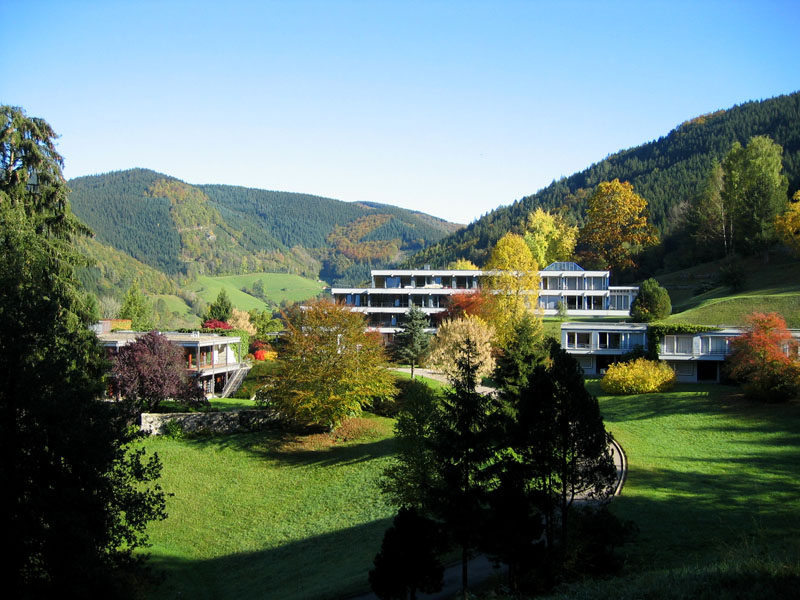
\includegraphics[width= 0.33 \textwidth]{mfo.jpg}
        \caption{An image scaled to 33\% of the textwidth.}
\label{fig:Institute}
\end{figure}

\begin{table}[ht]
  \caption{Jordan canonical form}
  \begin{tabular}{ l c r }
    17 & 1 & 0 \\
    0 & 17 & 0 \\
    0 & 0 & -3 \\
  \end{tabular}
  \label{tab:Jordan}
\end{table}

\subsection{A subsection}
\label{subsec:first}
More text and some formulas:
\begin{align}\label{real}
1+1&=2,\\\label{char.2}
1+1&=0.
\end{align}
Formula \eqref{real} refers to $\mathbb{R}$, Formula \eqref{char.2} does not\footnote{This is a footnote.\label{footnote}}.


\section{Another section heading}
\label{sec:another}

\subsection{Another subsection} \label{subsec:another}

\begin{figure}[ht]
        \centering 
        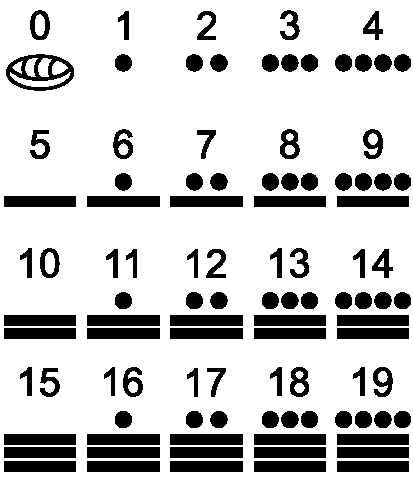
\includegraphics[width= 0.33 \textwidth]{maya.pdf}
        \caption{Exemplary image: Maya numerals.}
\label{fig:maya}
\end{figure}

\subsubsection{Sample subsubsection} \label{subsubsec:sample}

\newtheorem{theorem}{Theorem}
\begin{theorem}\label{thm:continuity}
Differentiability implies continuity.
\end{theorem}



\begin{imagecredits}
  \item[\autoref{fig:Institute}] Archives of the Mathematisches Forschungsinstitut Oberwolfach,\\\url{http://www.mfo.de}, 2004.
  \item[\autoref{fig:maya}] ``Maya''. Author: Bryan Derkson. Licensed under Creative Commons Attribution-Share Alike 3.0 via Wikimedia Commons, \url{http://commons.wikimedia.org/wiki/File:Maya.svg}, visited on \printdate{2014-09-05}.
\end{imagecredits}

\end{document}
